\chapter{Obsah přiloženého paměťového média}
\dirtree{%
.1 /.
.2 {.}git.
.2 {.}gitignore.
.2 Makefile.
.2 README.md\DTcomment{informace o projektu}.
.2 README.txt\DTcomment{návod na spuštění demo aplikací}.
.2 test.ps1\DTcomment{testovací PowerShell skript}.
.2 Data\DTcomment{složka se vzorovými daty}.
.2 Demo.
.3 CLI\DTcomment{konzolová demo aplikace (CLI)}.
.3 GUI\DTcomment{grafická demo aplikace (Windows)}.
.2 Images\DTcomment{složka s obrázky využitými v README.md}.
.2 Python\DTcomment{složka s python skripty referenčních filtrů}.
.2 Sources\DTcomment{složka se zdrojovými kódy}.
.3 NonlinearFilters.sln.
.3 NonlinearFilters.
.3 NonlinearFilters.APP.
.3 NonlinearFilters.APP.VolumeRenderer.
.3 NonlinearFilters.CLI.
.3 NonlinearFilters.Volume.
.2 Thesis\DTcomment{složka s textem práce napsaném v \LaTeX{u}}.
.3 project.pdf\DTcomment{PDF s textem bakalářské práce}.
.3 poster.pdf\DTcomment{plakát ve formátu A3}.
.3 \dots.
}

\chapter{Plakát}
\begin{figure} [H]
    \centering
    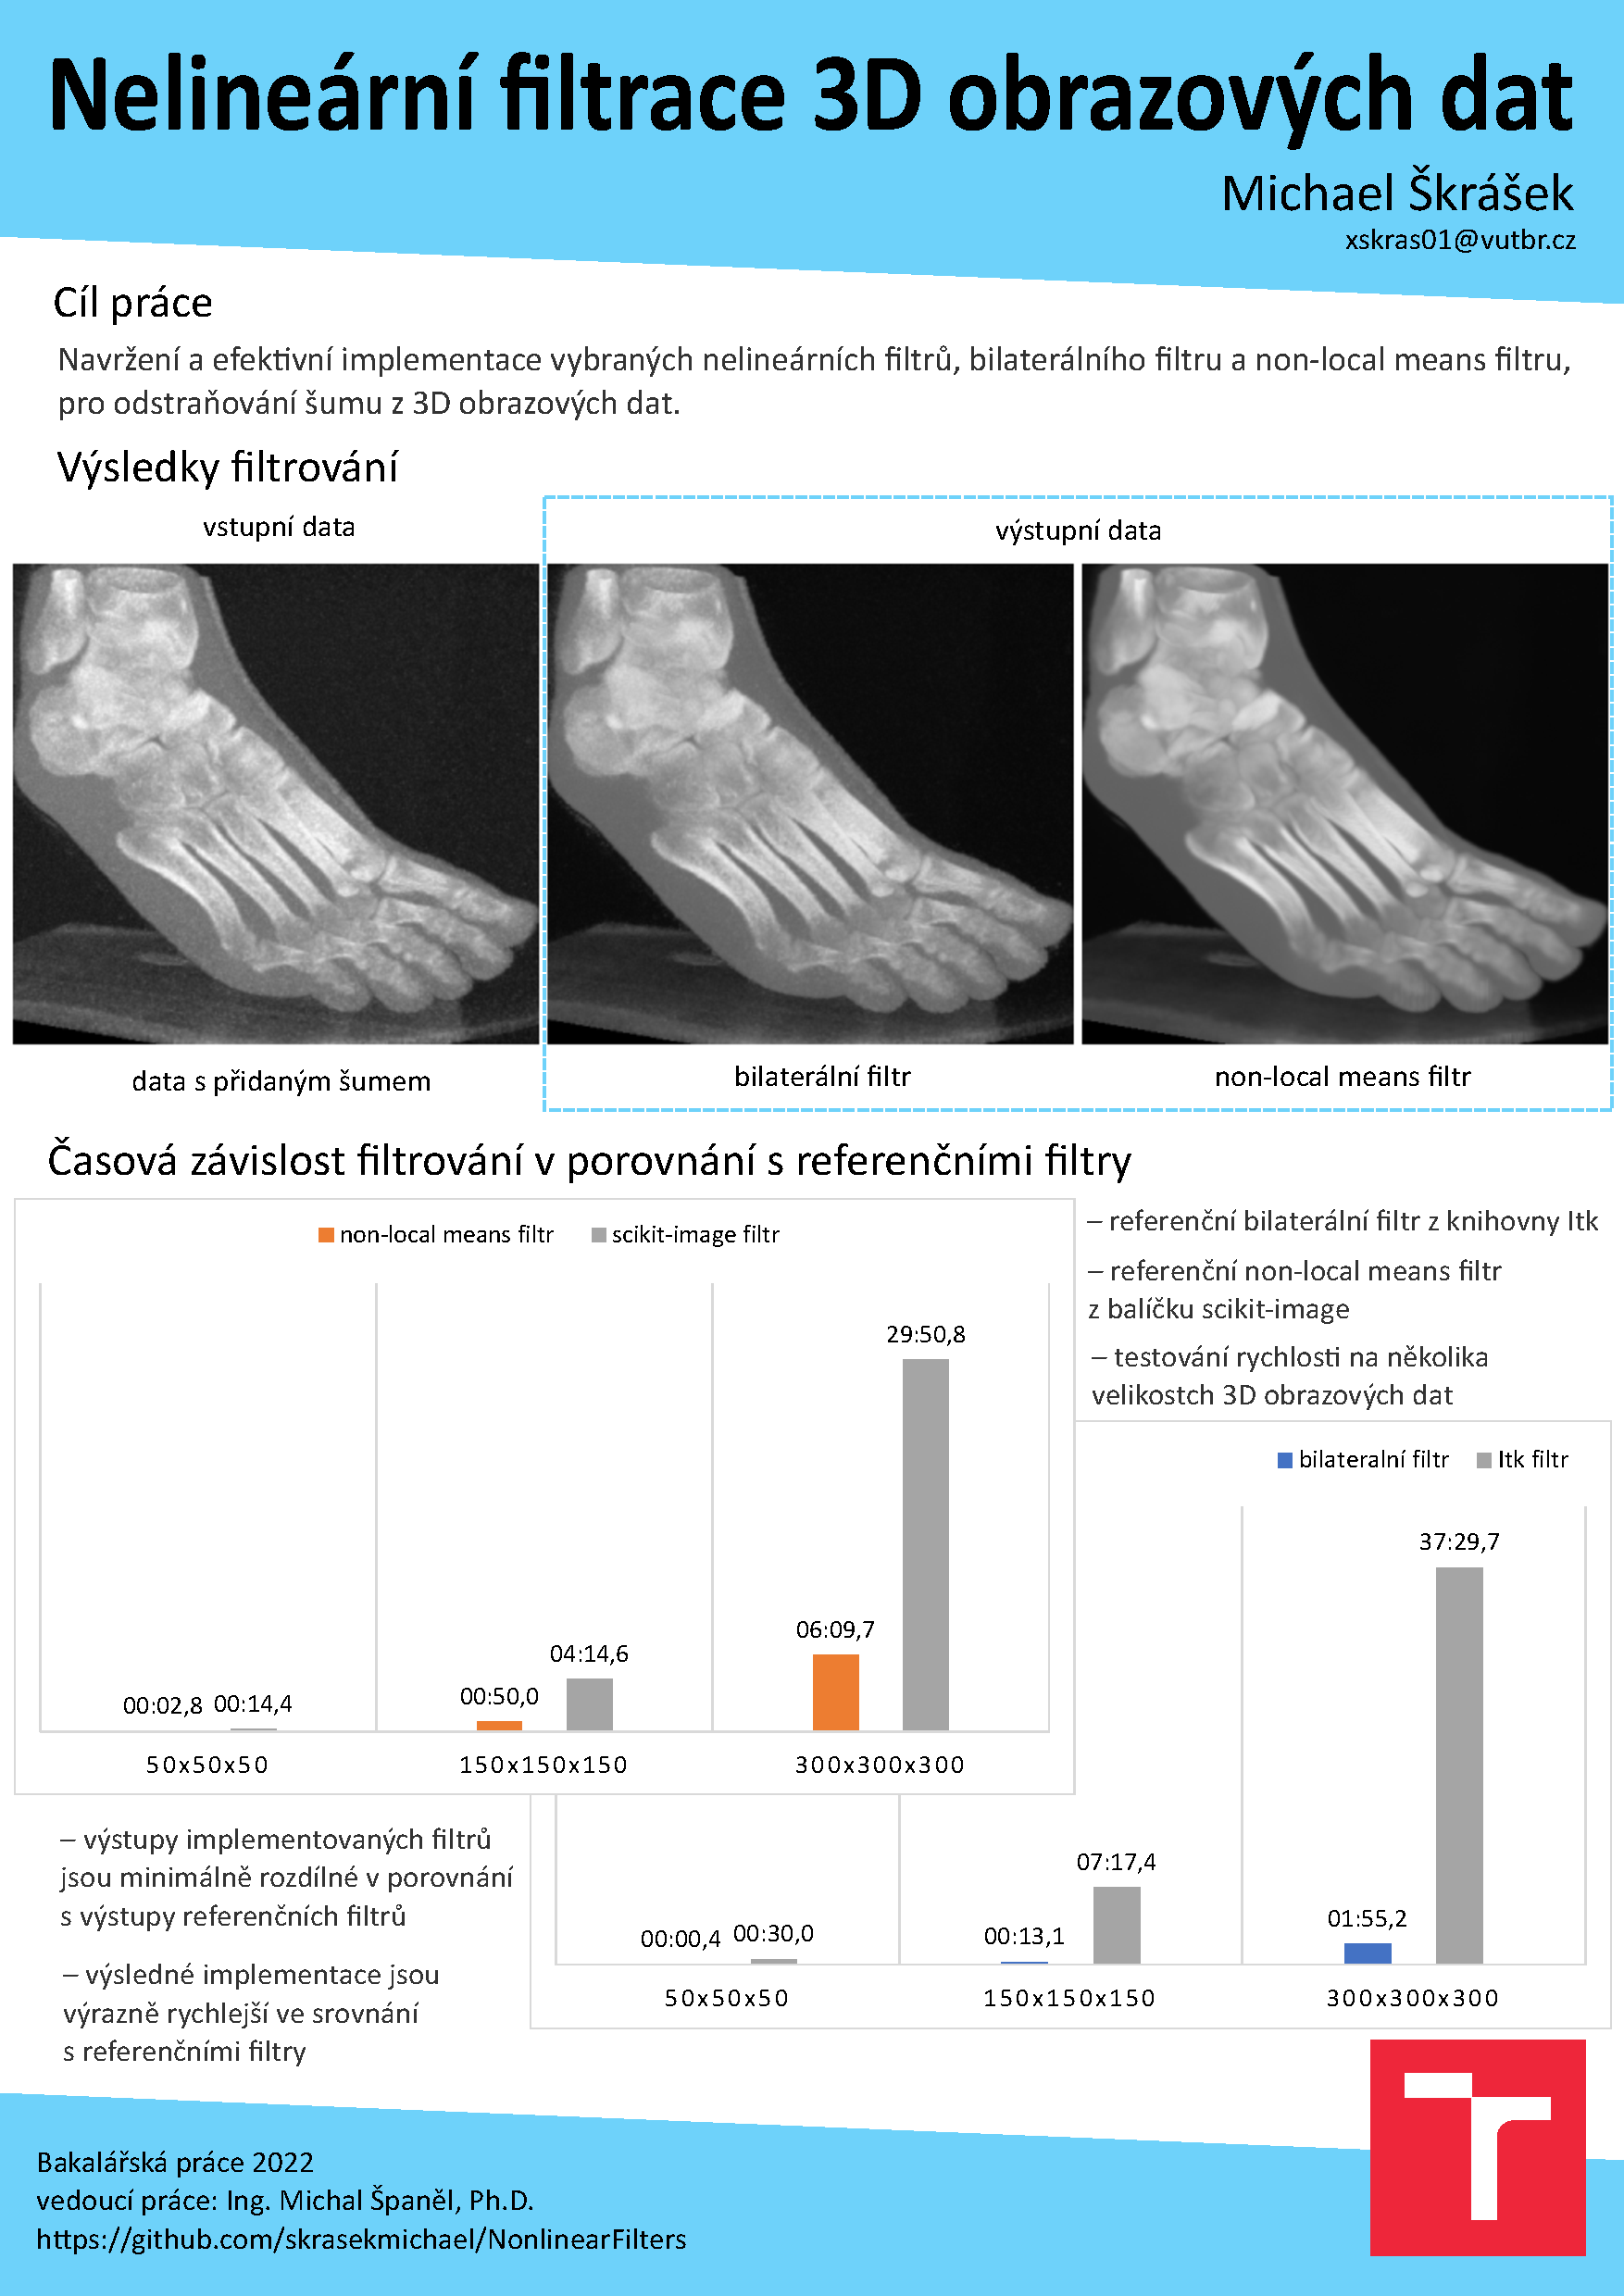
\includegraphics[width=0.7\textwidth]{poster.pdf}
    \caption{Ilustrace plakátu.}
\end{figure}
